\section{Further Properties of Linear Mappings}

\subsection{Adjoint Operators}

  \begin{definition}[Adjoint Operator]
    Let $A: U \longrightarrow V$ be a linear mapping between inner product spaces, with the inner product in $U$ and $V$ denoted $(\cdot,\cdot)_U$ and $(\cdot,\cdot)_V$, respectively. We can fix any $v \in V$ and define the linear function $l \in U^\ast$
    \begin{equation}
      l(\cdot) = \big(A(\cdot), v\big)_V
    \end{equation}
    Since $U$ is naturally isomorphic to $U^\ast$, we can define
    \begin{equation}
      l(\cdot) \equiv (\cdot, u^\prime)
    \end{equation} 
    to get 
    \begin{equation}
      \big(\cdot, u^\prime \big)_U \equiv \big(A(\cdot), v \big)_V
    \end{equation}
    By combining $(8)$, which defines an isomorphism between $U^\ast$ and $V$, and $(9)$, the natural isomorphism between $U$ and $U^\ast$, equation $(10)$ takes the composition of these to define an isomorphism from $V$ to $U$. This isomorphism is called the \textbf{adjoint} of $A$. 
    \begin{equation}
      A^\dagger: V \longrightarrow U, \;  \big(\; \cdot \;, A^\dagger v \big)_U = \big( A(\cdot), v \,\big)_V 
    \end{equation}
    By definition, given any $v \in V$, $A^\dagger v$ is defined so that the equality
    \begin{equation}
      (u, A^\dagger v) = (A u, v)
    \end{equation}
    holds for all values of $u \in U$. 
  \end{definition}

  It is important to note that the adjoint is not the same as the transpose since the transpose is a mapping between the dual spaces. Furthermore, the transpose is canonically defined upon defining the linear transformation $A: U \longrightarrow V$, while defining the adjoint requires the additional structure of an isomorphism from $U$ to $U^\ast$ and from $V$ to $V^\ast$. There are two ways to define these isomorphisms. 

  First, we can define dot products on both $U$ and $V$ and define the natural isomorphism 
  \begin{align*}
    &i: U \longrightarrow U^\ast, \; i(u) \equiv (u, \cdot) \in U^\ast\\
    &j: V \longrightarrow V^\ast, \; j(v) \equiv (v, \cdot) \in V^\ast
  \end{align*}
  This canonically creates the mapping 
  \begin{equation}
    i^{-1} A^T j: V \longrightarrow U
  \end{equation}
  which we define as the adjoint $A^\dagger$. This method using natural isomorphisms is precisely how we have defined the adjoint above. There is a second way, however. We can fix \textbf{orthonomal} bases on $U$ and $V$ and then assign them their respective dual spaces (satisfying the Kronecker delta function). Let the basis of $U$ be $\{u_1, ..., u_n\}$, $U^\ast$ be $\{u_1^\prime, ..., u_n^\prime\}$, $V$ be $\{v_1, ..., v_m\}$, and $V^\ast$ be $\{v_1^\prime, ..., v_m^\prime\}$. Now we can define the isomorphisms 
  \begin{align*}
    & i^\prime: U \longrightarrow U^\ast, \; i^\prime (u) \equiv c_1 u_1^\prime + ... + c_n u_n^\prime \\
    & j^\prime: V \longrightarrow V^\ast, \; j^\prime (v) \equiv k_1 v_1^\prime + ... + k_m v_m^\prime
  \end{align*}
  and then define the adjoint as 
  \begin{equation}
    A^\dagger \equiv i^{\prime -1} A^T j^\prime
  \end{equation}
  Let us compare these two definitions. Given a vector $u = a_1 u_1 + ... + a_n u_n, \Tilde{u} = b_1 u_1 + ... b_n u_n \in U$, 
  \begin{align*}
    &i(u)(\Tilde{u}) \equiv (u, \Tilde{u}) = \Big(\sum_{\alpha = 1}^n a_\alpha u_\alpha, \sum_{\beta = 1}^n b_\beta u_\beta \Big) = \sum_{\alpha, \beta} a_\alpha b_\beta \delta^\alpha_\beta = \sum_{\gamma=1}^n a_\gamma b_\gamma \\
    &i^\prime(u)(\Tilde{u}) \equiv \Big(\sum_{i=1}^n a_i u_i^\prime \Big) \Big( \sum_{j=1}^n b_j u_j \Big) = \sum_{i, j} a_i b_j u_i^\prime (u_j) = \sum_{i, j} a_i b_j \delta^i_j = \sum_{k=1}^n a_k b_k
  \end{align*}
  Similarly for vector $v = g_1 v_1 + ... g_n v_n, \Tilde{v} = h_1 v_1 + ... + h_n v_n \in V$, 
  \begin{align*}
    &i(v)(\Tilde{v}) \equiv (v, \Tilde{v}) = \Big(\sum_{\alpha = 1}^n g_\alpha v_\alpha, \sum_{\beta = 1}^n h_\beta v_\beta \Big) = \sum_{\alpha, \beta} g_\alpha h_\beta \delta^\alpha_\beta = \sum_{\gamma=1}^n g_\gamma h_\gamma \\
    &i^\prime(v)(\Tilde{v}) \equiv \Big(\sum_{i=1}^n g_i u_i^\prime \Big) \Big( \sum_{j=1}^n h_j v_j \Big) = \sum_{i, j} g_i h_j v_i^\prime (v_j) = \sum_{i, j} g_i h_j \delta^i_j = \sum_{k=1}^n g_k h_k
  \end{align*}
  Therefore, $i = i^\prime$ and $j = j^\prime$, meaning that the two derivations of the adjoint $A = i^{-1} A^T j = i^{-1 \prime} A^T j^\prime$ are exactly the same! We must note that the basis endowed on both $U$ and $V$ must be orthonormal for it to "mimic" the inner product. The derivation of the adjoint in these two equivalent methods may help the reader further understand that the adjoint $A^\dagger$ is really just a composition of fundamental linear functions $j: V \longrightarrow V^\ast$, $A^T: V^\ast \longrightarrow U^\ast$, and $i^{-1}: U^\ast \longrightarrow U$ that are all canonically created as soon as $A: U \longrightarrow V$ is created, along with the inner product spaces $U$ and $V$. 
  \begin{tikzcd}
    U \arrow{r}{A} \arrow{d}{i} & V \arrow{d}{j}\\
    U^\ast & V^\ast \arrow{l}{A^T}
  \end{tikzcd}

  However, it is hard to grasp a visual intuition of adjoint operators in general. Note that the properties of the transpose indicate that given $A: \mathbb{R}^n \longrightarrow \mathbb{R}^m$ with the standard orthonormal basis and dot product, the matrix representation of $A^\dagger$ is just $A^T$. If $A$ is a matrix over $\mathbb{C}$, then $A^\dagger$ is $A^H \equiv \bar{A}^T$, the \textbf{Hermitian transpose}, or \textbf{conjugate transpose}, of $A$. 

  Note that this definition of the adjoint of linear operators is completely unrelated to the definition of an adjoint of a matrix! 

  We now describe one common application of adjoints. 
  \begin{theorem}
    Let $A \in$ Mat$(m \times n, \mathbb{R})$ with $m > n$. This means that the system of equations $A x = p$ is an overdetermined system and will have no solutions with probability 1. However, we can find the \textbf{best-fit solution} of the system. That is, the vector $x$ that minimizes $\|A x -p\|^2$ is the solution $z$ of 
    \begin{equation}
      A^\dagger A z = A^\dagger p
    \end{equation}
    $z$ is therefore, the "closest approximation" of the solution of $A x = p$ that lives in $\mathbb{R}^n$. 
  \end{theorem}

  The QR decomposition is often used to simplify these linear least squares problems into a more manageable equation. 

  \begin{theorem}[QR Decomposition]
    Any real $m \times n$ matrix $A$ mapping $\mathbb{R}^n \longrightarrow \mathbb{R}^m$ may be decomposed as
    \begin{equation}
      A = QR
    \end{equation}
    where $Q$ is a $m \times n$ matrix with column vectors that are pairwise orthonormal and $R$ is an upper triangular square matrix. $Q$ having pairwise orthonormal columns $\implies Q^T Q = I$, so we can simplify the normal equation
    \begin{align*}
      A^T A x = A^T b & \implies (Q R)^T (Q R) x = R^T Q^T Q R x = R^T R x = R^T Q^T b \\
      & \implies R x = Q^T b \\
      & \implies x = R^{-1} Q^T b
    \end{align*}
  \end{theorem}

  \begin{theorem}
    Let $P_Y$ be the orthogonal projection onto $Y$. Then, 
    \begin{enumerate}
      \item $P_Y = P_Y^2$. 
      \item $P_Y = P_Y^\dagger$. 
    \end{enumerate}
  \end{theorem}

  \begin{theorem}[Properties of the Adjoint] Let $A, B: X \longrightarrow U, \; C: U \longrightarrow V$ be linear mappings. Then, 
    \begin{enumerate}
      \item $(A + B)^\dagger = A^\dagger + B^\dagger$
      \item $(C A)^\dagger = A^\dagger C^\dagger$
      \item $(A^{-1})^\dagger = (A^\dagger)^{-1}$ if $A$ is bijective
      \item $(A^\dagger)^\dagger = A$
    \end{enumerate}
  \end{theorem}

  \begin{definition}
    Linear mapping $A$ is \textbf{self adjoint} if and only if $A = A^\dagger$. If $M$ is any linear mapping, then its self-adjoint part is 
    \begin{equation}
      M_\delta = \frac{M + M^\dagger}{2}
    \end{equation}
  \end{definition}

  \begin{theorem}[Spectral Theorem]
    A $n$-dimensional self-adjoint map $H$ over $\mathbb{C}$ has real eigenvalues and an orthonormal basis of genuine eigenvectors. That is, its eigendecomposition consists of $n$ pairwise orthogonal eigenspaces. 
  \end{theorem}

  \begin{corollary}
    Given a real self-adjoint matrix $H$, there exists a real invertible matrix $M$ such that $M^\dagger H M = D$, with $D$ diagonal and the column vectors form an orthonormal basis.

    So, given self-adjoint $H: X \longrightarrow X$, the whole space can be written as the direct sum of pairwise orthogonal eigenspaces. 
    \begin{equation}
      X = \bigoplus_{i=1}^n E(\lambda_i)
    \end{equation}
    which implies that every $x \in X$ can be written uniquely as 
    \begin{equation}
      x = x_1 + x_2 + ... + x_n, \; x_i \in E(\lambda_i) 
    \end{equation}
  \end{corollary}

  \begin{definition}
    Given that $P_j$ is the orthogonal projection onto the $j$th eigenspace $E(\lambda_j)$, that is
    \begin{equation}
      P_j (x) = x_j \in E(\lambda_j), \; \text{ ($P_j$ also self adjoint)}
    \end{equation}
    the \textbf{spectral resolution} of self-adjoint mapping $H$ is the decomposition into the form 
    \begin{equation}
      H = \sum_j \lambda_j P_j \implies H x = \bigg( \sum_j \lambda_j P_j \bigg) x = \sum_j \lambda_j x_j
    \end{equation}
    The resolution of the identity is
    \begin{equation}
      I = \sum_j P_j
    \end{equation}
  \end{definition}

  \begin{proposition}
    Given the spectral resolution of self-adjoint $H$, 
    \begin{equation}
      H  = \sum_j \lambda_j P_j \implies H^2 = \sum_j \lambda_j^2 P_j
    \end{equation}
  \end{proposition}

  Note that the spectral resolution of a self adjoint mapping is precisely the eigendecomposition of the mapping into its 1-dimensional eigenspaces. It is merely a simpler form of the eigendecomposition in the specific case when the linear mapping is self-adjoint. 

  \begin{theorem}
    Let $H, K$ be self-adjoint mappings such that $H K = K H$. Then $H$ and $K$ have the same spectral resolution, i.e. they have the same eigendecomposition. 
    \begin{equation}
      H = \sum_j a_j P_j, \; \; K = \sum_j b_j P_j
    \end{equation}
  \end{theorem}
  \begin{proof}
    $x \in E(a) H x = a x \implies K H x = a K x \implies H K x = a K x \implies K x \in E(a)$. Similarly, we can do this with $K$ to find $x \in E(a) \implies H x \in E(a)$, meaning that $K$ and $H$ have the same eigendecompositions (though their eigenvalues are not necessarily equal). 
  \end{proof}

  \begin{definition}[Anti-Self-Adjoint]
    Map $A$ is \textbf{anti-self adjoint} if $A^\dagger = - A$. Conjugate symmetry implies that
    \begin{equation}
      A^\dagger = A \iff (i A)^\dagger = - (i A)
    \end{equation}
    So, given an anti-self adjoint map $A$, we can apply the spectral resolution to $iA$. 
  \end{definition}

  \begin{theorem}
    Given anti-self adjoint $A: \mathbb{C}^n \longrightarrow \mathbb{C}^n$, 
    \begin{enumerate}
      \item eigenvalues of $A$ are purely imaginary
      \item we can choose an orthonormal basis of eigenvectors of $A$
    \end{enumerate}
  \end{theorem}
  \begin{proof}
    This easily follows from the Spectral Theorem. 
  \end{proof}

  \begin{definition}[Normal Maps]
    $N: X \longrightarrow X$ is a \textbf{normal mapping} if $N^\dagger N = N N^\dagger$. Self-adjoint, anti-self adjoint, and unitary matrices are all normal. Surprisingly, the set of normal matrices are not closed under addition nor multiplication, so they do not form a group. 
  \end{definition}

  \begin{theorem}
    A map $N$ is normal if and only if it has an orthonormal basis of eigenvectors, i.e. it is unitarily diagonalizable. That is, 
    \begin{equation}
      N = U^\dagger D U 
    \end{equation}
  \end{theorem}
  \begin{proof}
    $(\rightarrow)$ Let 
    \begin{equation}
      H = \frac{1}{2} (N + N^\dagger), \; A = \frac{1}{2} (N - N^\dagger)
    \end{equation}
    $N^\dagger N = N N^\dagger \implies A H = H A$, where $H$ is self adjoint, $A$ is anti-self adjoint, and $N = H + A, N^\dagger = H - A$. Since $A H = H A$, they have the same spectral resolution of orthonormal eigenspaces, which also forms the same spectral resolution for $N = H + A$. \\
    $(\leftarrow)$ $A = U^\dagger D U \implies A^\dagger A = (U^\dagger D U) (U^\dagger \bar{D} U) = U^\dagger D \bar{D} U = A A^\dagger$. 
  \end{proof}

\subsection{Lie Groups and the Exponential Map}

  \begin{definition}[General Linear Group]
    Aut$(V)$ of vector space $V$ also forms a group under composition. We denote it GL$(V)$. The group of automorphisms of $\mathbb{R}^n$ and $\mathbb{C}^n$ is denoted GL$(\mathbb{R}^n)$ and GL$(\mathbb{C}^n)$, respectively. The group of all invertible $n \times n$ matrices over $\mathbb{R}$ and $\mathbb{C}$ is denoted GL$_n(\mathbb{R})$ and GL$_n(\mathbb{C})$. GL$_n(\mathbb{R})$ is also denoted GL$(n, \mathbb{R})$, and similarly for GL$(n, \mathbb{C})$. 
  \end{definition}

  \begin{proposition}
    Given that $V$ is a real vector space, 
    \begin{equation}
      GL(V) \simeq GL(\mathbb{R}^n) \simeq GL_n (\mathbb{R})
    \end{equation}
    since GL$_n(\mathbb{R})$ are representations of linear operators. Similarly, if $V$ is a complex vector space, 
    \begin{equation}
      GL(V) \simeq GL(\mathbb{C}^n) \simeq GL_n (\mathbb{C})
    \end{equation}
  \end{proposition}

  \begin{definition}[Special Linear Group]
    The group of all real $n \times n$ matrices that have determinant $1$ is called the \textbf{special linear group}, denoted SL$_n (\mathbb{R})$. It is a subgroup of GL$_n (\mathbb{R})$. The group of all complex $n \times n$ matrices with determinant $1$ is denoted SL$_n (\mathbb{C})$. It is a subgroup of GL$_n(\mathbb{C})$. 
  \end{definition}

  \begin{definition}[Isometry]
    An \textbf{isometry} $M$ of metric space $(X, d)$ is a mapping that preserves all distances. That is, for all $x, y \in X$, 
    \begin{equation}
      d(x, y) = d(M x, M y) 
    \end{equation}
    The set of all isometries, denoted Isom$(X)$, is a group that is generated by all translations, rotations, and reflections. 
  \end{definition}

  Since linear maps always preserve the origin, we will focus on origin-preserving isometries, which is a subgroup called the orthogonal group.

  \begin{definition}[Orthogonal Group]
    The \textbf{orthogonal group} of a real Euclidean space of dimension $n$, denoted $O(n)$, is the group of all origin-preserving isometries of the space consisting of rotations and reflections. The matrix representation of this group is the set of real $n \times n$ matrices where the column vectors form an orthonormal basis. Note that the determinant of every element of $O(n)$ is $\pm 1$. 
  \end{definition}

  \begin{definition}[Orthogonal Matrix]
    An \textbf{orthogonal matrix} is the matrix representation of an element in $O(n)$. It is the real $n \times n$ matrix where all the column vectors are pairwise orthogonal and all have magnitude 1. 
  \end{definition}

  \begin{proposition}
    The rows of an orthogonal matrix are also pairwise orthonormal.
  \end{proposition}

  \begin{proposition}
    Given an orthogonal matrix $M$,
    \begin{equation}
      M^T = M^{-1}
    \end{equation}
  \end{proposition}

  \begin{definition}[Special Orthogonal Group]
    The \textbf{special orthogonal group} of a real Euclidean space of dimension $n$, denoted $SO(n)$, is the group of all isometries that preserve the handedness of the space consisting only of rotations. It is a subgroup of $O(n)$. The matrix representation of this group is the set of real $n \times n$ matrices where the column vectors are pairwise orthonormal and the determinant $=1$. 
  \end{definition}

  We extend this concept to complex Euclidean spaces. 

  \begin{definition}[Unitary Group]
    The \textbf{unitary group of degree $n$} is the group of all complex $n \times n$ matrices where the columns are pairwise orthogonal. It is denoted $U(n)$. 
  \end{definition}

  \begin{example}
    $U(1)$ is the set of complex numbers with norm $1$. 
  \end{example}

  \begin{definition}[Special Unitary Group]
    The \textbf{special unitary group of degree $n$} is the group of all complex $n \times n$ matrices where the columns are pairwise orthogonal and determinant $=1$. It is denoted $SU(n)$. 
  \end{definition}

  The groups mentioned in this section are examples of \textit{Lie Groups}. Lie groups in general will not be defined in here, since they require knowledge of smooth manifolds and differential geometry. In order to analyze these abstract groups, we use the exponential map $e \in$ End$($ Mat$(n, \mathbb{F})$ to reduce these Lie groups to Lie algebras.

\subsection{Singular Values, Norms of Linear Mappings}

  Since the algebra of linear operators is itself a vector space, we can also define structures on it, too. We focus on matrix norms. 

  \begin{definition}[Operator Norm]
    Let $A: X \longrightarrow U$ be linear. Then, we define
    \begin{equation}
      \|A\| = \sup_{\|x\|=1} \|A x\|
    \end{equation}
    Note that $\|A x\|$ is measure with respect to the norm of $U$ and $\|x\|$ the norm of $X$. 
  \end{definition}

  There is a very nice visualization of this. 

  \begin{figure}[H]
    \centering 
    \begin{tikzpicture}
      % Left diagram (Unit circle in R^n)
      \begin{scope}[shift={(-4,0)}]
        % Axes
        \draw[-] (-2.5,0) -- (2.5,0);
        \draw[-] (0,-2.5) -- (0,2.5);
        
        % Unit circle
        \draw[thick] (0,0) circle (1.5cm);
        
        % Label R^n
        \node at (0.8,2) {$\mathbb{R}^n$};
      \end{scope}
      
      % Arrow with label A
      \draw[-{Stealth[length=3mm,width=2mm]}] (-1.5,0.5) -- (1.5,0.5);
      \node at (0,1) {$A$};
      
      % Right diagram (Ellipse in R^m)
      \begin{scope}[shift={(4,0)}]
        % Axes
        \draw[-] (-2.5,0) -- (2.5,0);
        \draw[-] (0,-2.5) -- (0,2.5);
        
        % Rotated Ellipse (30 degrees)
        \draw[thick, rotate=30] (0,0) ellipse (2cm and 1cm);
        
        % Major axis line
        \draw[->, thick, rotate=30] (0,0) -- (2,0);
        
        % Label R^m
        \node at (1.8,2) {$\mathbb{R}^m$};
      \end{scope}
    \end{tikzpicture}
    \caption{The norm of $A$ is the length of the major axis of the ellipsoid. Given that $\dim{X}=n$, imagine the $n$-dimensional unit ball in $X$ being transformed under $A$. The image of the ball should be an ellipsoid (of dimension $\leq m$) in $U$. } 
    \label{fig:operator_norm}
  \end{figure}

  \begin{theorem}
    \begin{align}
      \|A z\| \leq \|A\| \|z\| \text{ for all } z \in X \\
      \|A\| = \sup_{\|x\|, \|v\| = 1} (A x, v)
    \end{align}
  \end{theorem}
  \begin{proof}
    \begin{align*}
      &\|A z\| \leq \sup{\|A z\|} = \sup{\Big|\Big| A \frac{z}{\|z\|} \Big|\Big|} = \|A\| \|z\| \\
      &\|u\| \equiv \max_{\|v\|=1} (u, v) \implies \|A x\| \equiv \max_{\|v\|=1} (Ax, v) \implies \|A\| \equiv \sup_{\|x\|, \|v\| =1} (A x, v)
    \end{align*}
  \end{proof}

  \begin{theorem}[Properties of Matrix Norm]
    Let there exist any $k \in \mathbb{F}$, with any $A, B: X \longrightarrow U$, $C: U \longrightarrow V$. Then, 
    \begin{enumerate}
      \item $\|k A\| = |k| \|A\|$
      \item $\|A + B\| \leq \|A\| + \|B\|$
      \item $\|C A\| \leq \|C\| \|A\|$
      \item $\|A\| = \|A^\dagger\|$
    \end{enumerate}
  \end{theorem}

  \begin{definition}[Spectral Radius]
    The \textbf{spectral radius} of $A$ is defined
    \begin{equation}
      r(A) \equiv \max_i |a_i|, \; a_i \text{ are eigenvalues}
    \end{equation}
  \end{definition}

  \begin{proposition}
    A simple lower and upper bound of $\|A\|$ can be defined
    \begin{equation}
      r(A) \leq \|A\| \leq \bigg( \sum_{i, j} a_{i j}^2 \bigg)^\frac{1}{2}
    \end{equation}
  \end{proposition}

  Matrix norms have extremely useful applications in determining the existence of invereses. 

  \begin{theorem}
    Let $A$ be invertible and 
    \begin{equation}
      \|A - B\| < \frac{1}{\|A^{-1}\|}
    \end{equation}
    in the sense that $B$ is "close" to $A$. Then $B$ is invertible. 
  \end{theorem}

  We now proceed to another crucial decomposition, called the singular value decomposition. While the JNF allows us to choose the most convenient choice of basis for a square matrix, the Singular Value Decomposition (SVD) allows us to decompose general $m \times n$ matrices. 

  \begin{theorem}[Singular Value Decomposition]
    Any linear mapping $M$ from an $n$-dimensional inner product space to a $m$-dimensional inner product space can be decomposed into 
    \begin{equation}
      M = U \Sigma V^\dagger = \begin{pmatrix}
       \vert & \vert & \vert & \vert\\
      y_1 & y_2 & \ldots & y_m \\
      \vert & \vert & \vert & \vert
      \end{pmatrix}\begin{pmatrix}
      \sigma_1 & & & &0\\
      &\ddots &&& \vdots \\
      & & \sigma_p & & 0\\
      & & & \ddots &\vdots \\
      0 & \ldots &0& \ldots &0
      \end{pmatrix} \begin{pmatrix}
      \text{---}&x_1&\text{---} \\
      \text{---}&x_2&\text{---} \\
      \text{---}&\vdots&\text{---} \\
      \text{---}&x_n&\text{---}
      \end{pmatrix}
    \end{equation}
    where $U \in U(m), V \in U(n)$ and $\Sigma$ has diagonal elements with nonnegative real entries. Also, $p = $ rank$(M) \leq \min{\{n,m\}}$. This form is known as the \textbf{singular value decomposition}. The columns of $U$, denoted $y_i$, are called the \textbf{left singular vectors} and the columns of $V$ (i.e. the rows of $V^\dagger$), denoted $x_i$, are called the \textbf{right singular vectors}. The diagonal entries of $\Sigma$ are called the \textbf{singular values}. The SVD is unique up to the order of singular values, but it is generally constructed so that $\sigma_1 \geq \sigma_2 \geq \ldots \geq \sigma_p$. 
  \end{theorem}

  To provide a brief, yet unrigorous, justificiation of why the SVD exists, we look at the linear mapping $M: X \longrightarrow Y$, with $\dim{X} = n, \dim{Y} = m$. If $M$ is injective $(\iff m \geq n)$, given the basis $\{e_i\}$ for $X$, we can complete the linearly independent set $\{Me_i\}_{i=1}^n$ to a basis in $Y$ and represent $M$ as the mapping
  \begin{equation}
    \Sigma_{inj} = \begin{pmatrix} &&\\ &I_n&\\ &&\\ 0&\ldots &0 \end{pmatrix}
  \end{equation}
  If $M$ is surjective $(\iff m \leq n)$, then given basis $\{f_i\}_{i=1}^m$ of $Y$, we can choose a basis $\{e_j\}_{j=1}^n$ of $X$ such that $M(e_i) = f_i (i = 1, 2, \ldots, m)$, and $M(e_i) = 0$ when $i > m$. This produces the matrix
  \begin{equation}
    \Sigma_{surj} = \begin{pmatrix} &&&0\\&I_m&& \vdots \\&&&0\end{pmatrix}
  \end{equation}
  We now present the following theorem without proof. 

  \begin{theorem}
    Any map $M: X \longrightarrow Y$ can be written as a surjective map followed by an injective map. 
  \end{theorem}

  This theorem implies that any map, when given the right choice of basis, can be written as 
  \begin{equation}
    \Sigma_{inj} \Sigma_{surj} = \begin{pmatrix}
    &&&...&0\\
    &I_p&&...&0\\
    &&&...&...\\
    ...&...&...&...&0\\
    0&0&...&0&0
    \end{pmatrix} = \begin{pmatrix}
    1&&&&0\\
    &...&&&...\\
    &&1&&0\\
    &&&...&...\\
    0&...&0&...&0
    \end{pmatrix}
  \end{equation}
  where rk$(M) = p = $ the number of $1$'s in $\Sigma_{inj} \Sigma_{surj}$. As for choosing the proper set basis for $X$ and $Y$, we can find these passive transformations in the unitary groups $U(n)$ and $U(m)$. 

  We now present a geometric description of the singular value decomposition. Think of the unit $n$-ball being rotated and flipped ($V^\dagger$ applied) under the unitary transformation. Then, it is stretched along its othogonal axes to result in an ellipsoid living in an $m$-dimensional space. The factor of stretching and compressing the axes are precisely the singular values. Finally, this ellipsoid is rotated and flipped ($U$ applied) back to its original basis. 

  \begin{theorem}
    Geometrically, we can see that the largest singular value is the matrix norm, also called the operator norm. 
    \begin{equation}
      \|M\| = \sigma_1
    \end{equation}
  \end{theorem}

  \begin{theorem}[Properties of Singular Values] 
    Given linear mapping $A$ from a $n$-dimensional inner product space to $m$-dimensional inner product space, 
    \begin{enumerate}
      \item $\sigma_i(A) = \sigma_i (A^T) = \sigma_i (A^\dagger) = \sigma_i (\bar{A})$

      \item $\forall \; U \in U(m), V \in U(n), \; \sigma_i (A) = \sigma_i (U A V)$

      \item Relation to eigenvalues
      \begin{equation}
        \sigma_i^2(A) = \lambda_i (A^\dagger A) = \lambda_i (A A^\dagger)
      \end{equation}
    \end{enumerate}
  \end{theorem}

  We now present the (not the best) process of computing SVD of small matrices by hand. Given matrix $M$, $M = U \Sigma V^\dagger \implies M^\dagger M = V \Sigma^2 V^\dagger$. The eigenvalues of $M^\dagger M$ are $\sigma_i^2$ with corresponding eigenvectors being the columns of $V$, which can all be found by putting $M^\dagger M$ into JNF. We repeat this process for $M M^\dagger = U \Sigma^2 U^\dagger$ to find the eigenvectors that make up the column vectors of $U$. 

  \begin{theorem}
    Let $A: X \longrightarrow Y$, with $\dim{X} = n, \dim{Y} = m$, and let $k \leq \min{\{m, n\}}$, with $A = U \Sigma V^\dagger$. Then, amongst all rank $k$ $m \times n$ matrices $B$, the matrix $A^{(k)}$ minimizes 
    \begin{equation}
      \|A-B\|_2, \; A^{(k)} = U \Sigma^{(k)} V^\dagger
    \end{equation}
    and $\Sigma^{(k)}$ is $\Sigma$ with $\sigma_{k+1} = \sigma_{k+2} = ... = 0$. Therefore, to see how "close" $B$ is to $A$, we can compare the singular values of $A$ and $B$, given that they both have the same unitary matrices $U$ and $V$. 
  \end{theorem}

  The singular value decomposition has many applications in high dimensional data analysis and data compression. For example, in a set of $m$ data points in $\mathbb{R}^n$ that each lie in the rows of matrix $A$, if the singular values of $A$ suddenly drops (e.g. 120, 118, 107, 98, 2, 1, 0.3, ...) then we can determine that the points "almost" lie in a subspace in $\mathbb{R}^n$. Knowing this allows us to compress high dimensional data to $A^{(k)}$, which is a more manageable form. This is especially useful in the data compression of electronic images, where each pixel is treated as a single number to form a matrix. 

  It can also be used to define the "pseudo-inverse" of a matrix that may not be invertible. 

  \begin{definition}[Pseudo-Inverse]
    Given matrix $M = U \Sigma V^\dagger$ in SVD, we define the \textbf{pseudo-inverse} $M^+ = V \Sigma^+ U^\dagger$, where $\Sigma^+$ is $\Sigma$ with entries $\sigma_i^{-1}$, or $0$ if $\sigma_i = 0$. For example,
    \begin{equation}
      \Sigma = \begin{pmatrix}3&0&0\\0&2&0\\0&0&0\end{pmatrix} \implies \Sigma^+ = \begin{pmatrix}1/3&0&0\\0&1/2&0\\0&0&0\end{pmatrix}
    \end{equation}
    $\implies M^+ M = V \Sigma^+ \Sigma V^\dagger$. If $M$ is square and all $\sigma_i \neq 0$, then $M^\dagger M = V V^\dagger \implies M^\dagger M = I \implies  M^+ = M^{-1}$. 
  \end{definition}

  By computing the SVD of $M$, where $\sigma_p \neq 0, p =$ rk$\,M = $ rk$\,\Sigma$, we can automatically compute the 4 fundamental spaces. 
  \begin{equation}
    M = U \Sigma V^\dagger = \begin{pmatrix}&&&&|&\\&&&&|&\\&&U&&|&U^\prime\\&&&&|&\\&&&&|&
    \end{pmatrix} \begin{pmatrix}
    \sigma_1&&&&0\\
    &\sigma_2&&&0\\
    &&...&&...\\
    &&&\sigma_p&0\\
    0&0&...&0&0
    \end{pmatrix}\begin{pmatrix}
    &&&&\\&&&&\\&&V^\dagger&&\\&&&&\\\text{---}&\text{---}&\text{---}&\text{---}&\text{---}
    \\&&V^{\dagger \prime}&&
    \end{pmatrix}
  \end{equation}
  \begin{enumerate}
    \item $\im{M} = C(U)$
    \item $\ker{M} = R(V^{\dagger \prime}) = C(V^\prime)$
    \item $\ker{M^\dagger} = C(U^\prime)$
    \item $\im{M^\dagger} = C(V) = R(V^\dagger)$
  \end{enumerate}

  One of the main differences between the JNF and SVD of a matrix $A$ lies in how they are affected by perturbations in the elements of $A$. For example, take the small change 
  \begin{equation}
    A = \begin{pmatrix}
    1 & 1\\
    0 & 1
    \end{pmatrix} \longrightarrow A^\prime  = \begin{pmatrix}
    1 & 1 \\
    0 & 1.00001
    \end{pmatrix}
  \end{equation}
  The SVD of $A^\prime$ will "change" continuously for changes in the elements of $A$, but the JNF of $A$ is completely different from the JNF of $A^\prime$. More specifically, the JNF of $A$ is $A$ itself, but the JNF os $A^\prime$ is now diagonalizable, meaning that the 2-dimensional eigenspace $E(1)$ "breaks up" into two 1-dimensional eigenspaces from small perturbations. 

  \begin{definition}[Frobenius Norm]
    The \textbf{Frobenius norm} of a $m \times n$ matrix $A$ is defined
    \begin{equation}
      \|A\|_F \equiv \sqrt{\Tr{(A^\dagger A)}} = \sqrt{\Tr{\Sigma^2}} = \bigg( \sum_{i, j} a_{i j}^2 \bigg)^{\frac{1}{2}} 
    \end{equation}
    By Singular Value Decomposition, we can reduce its calculations to
    \begin{equation}
      \|A\|_F = \sqrt{\sum_i \sigma_i^2}
    \end{equation}
    where $\sigma_i$'s are the singular values. Clearly, 
    \begin{equation}
      \|A\|_2 \leq \|M\|_F
    \end{equation}
    In quantum mechanics, the Frobenius norm is also called the \textbf{Hilbert Schmidt norm} in the context of infinite dimensional Hilbert spaces. 
  \end{definition}

  We end by defining two more common decompositions of square matrices. 

  \begin{theorem}[Schur Decomposition]
    Every $n \times n$ matrix $A$ over $\mathbb{C}$ can be decomposed into
    \begin{equation}
      A = Q T Q^\dagger
    \end{equation}
    where $Q \in U(n)$ and $T$ is upper triangular. 
  \end{theorem}
  \begin{proof}
    This is an obvious result of the Grahm-Schmidt algorithm. 
  \end{proof}

  \begin{theorem}[Polar Decomposition]
    Every complex $n \times n$ matrix $A$ can be factored into the form
    \begin{equation}
      A = U P
    \end{equation}
    where $U \in U(n)$ and $P$ is a positive semidefinite self-adjoint matrix. If $A$ is a real matrix, then $U \in O(n)$. 
  \end{theorem}
  \begin{proof}
    We take the SVD to get 
    \begin{equation}
      A = W \Sigma V^\dagger
    \end{equation}
    and we can assign 
    \begin{equation}
      U = W V^\dagger, \; P = V \Sigma V^\dagger
    \end{equation}
    Since $V, W$ are unitary, this confirms that $P$ is positive definite and self-adjoint along with $U$ being unitary. Thus, the existence of the SVD implies the existence of the polar decomposition. 
  \end{proof}

\subsection{Positive Definite Matrices}

  \begin{definition}[Positive-Semidefinite]
    A self-adjoint linear mapping $H$ from a real or complex Euclidean space onto itself is \textbf{positive definite} if 
    \begin{equation}
      (x, H x) > 0 \text{ for all } x \neq 0
    \end{equation}
    $H$ is called \textbf{positive semidefinite} if 
    \begin{equation}
      (x, H x) \geq 0
    \end{equation}
  \end{definition}

  \begin{theorem}[Polar Decomposition]
    Given a Euclidean space $\mathbb{E}^n$ and any linear endomorphism $f$ of $\mathbb{E}^n$, there are two positive definite self-adjoint linear maps $h_1, h_2 \in$ End$(\mathbb{E}^n)$ and $g \in$ O$(n)$ such that
    \begin{equation}
      f = g \circ h_1 = h_2 \circ g
    \end{equation}
    That is, such that $f$ can be decomposed into the following as shown in this commutative diagram. 
    \begin{tikzcd}
      \mathbb{E}^n \arrow{r}{h_2} & \mathbb{E}^n \\
      \mathbb{E}^n \arrow{u}{g} \arrow{ur}{f} \arrow{r}{h_1} & \mathbb{E}^n \arrow{u}{g}
    \end{tikzcd}
  \end{theorem}

  \begin{theorem}[Properties of Positive Definite Matrices] 
    Here we state basic properties. 
    \begin{enumerate}
      \item $I$ is positive definite. 
      \item Positive mappings form a subspace in the space of linear mappings. 
      \begin{align*}
        &M, N \text{ positive} \implies M + N \text{ is positive} \\
        &M \text{ positive} \implies a M \text{ is positive for all} a \in \mathbb{F}
      \end{align*}
      \item $H$ positive and $Q$ invertible $\implies Q^\dagger H Q$ positive. 
    \end{enumerate}
  \end{theorem}

  \begin{theorem}
    $H$ is positive definite if and only if all of its eigenvalues are positive. Furthermore, every positive mapping is invertible.
  \end{theorem}

  \begin{theorem}
    Every positive mapping $M$ has a unique positive square root. That is, there exists a unique positive mapping $N$ such that
    \begin{equation}
      N^2 = M 
    \end{equation}
    We denote $N$ as $\sqrt{M}$. 
  \end{theorem}

  \begin{definition}
    Given that $M, N$ are positive definite mappings. 
    \begin{equation}
      M > N \iff M - N > 0, \text{ that is, $M$ is positive}
    \end{equation}
  \end{definition}

  \begin{theorem}
    If $M, N$ are positive definite mappings 
    \begin{equation}
       M > N \implies M^{-1} < N^{-1}
    \end{equation}
  \end{theorem}

  \begin{proposition}
    In $\mathbb{R}^n$ endowed with the dot product, a $n \times n$ matrix $A$ is positive definite if and only if 
    \begin{equation}
      (x, A y) = x^T A y > 0 
    \end{equation}
    for every $x, y \in \mathbb{R}^n$. $A$ is positive semi-definite if and only if 
    \begin{equation}
      (x, A y) = x^T A y \geq 0
    \end{equation}
  \end{proposition}

  The following is a useful fact regarding inner products of $\mathbb{R}^n$. 

  \begin{proposition}
    The set of all inner products that can be defined on $\mathbb{R}^n$ is bijective to the set of positive-definite symmetric $n \times n$ matrices $A$ (which is itself bijective to the set of all positive-definite mappings). That is, every inner product of $\mathbb{R}^n$ can be defined 
    \begin{equation}
      (x, y) \equiv x^T A y
    \end{equation}
    Note that when $A = I_n$, the inner product is the regular dot product.
  \end{proposition}

\subsection{Stochastic Matrices, Markov Chains}

  \begin{definition}[Entrywise Positive]
    A real $n \times n$ matrix $P$ is \textbf{entrywise positive} if all entries are positive real numbers. We similarly define entrywise positive vectors having components as positive real numbers. With this notion of positiveness. We can define
    \begin{equation}
      A > B \iff A - B > 0 \iff (A-B)_{i j} > 0 \; \forall i, j
    \end{equation}
  \end{definition}

  Note that this definition of positive matrices is \textit{not} the same as positive-definite matrices! 

  \begin{theorem}[Perron's Theorem]
    Every entrywise positive matrix $P$ has a real \textbf{dominant eigenvalue}, denoted $\lambda(P) \in \mathbb{R}$ satisfying
    \begin{enumerate}
      \item $\lambda(P) > 0$, and the associated eigenvector $h >0$
      \item $\lambda(P)$ is a simple eigenvalue
      \item every other eigenvalue $\kappa$ satisfies: $|\kappa| < \lambda(P)$
      \item there is no other eigenvector $\geq 0$, i.e. all other eigenvectors have at least 1 negative entry.
    \end{enumerate}
  \end{theorem}

  \begin{definition}[Stochastic Matrix]
    A \textbf{stochastic matrix} is a matrix $A$ where the elements of each column $a_i$ sum up to $1$. $A$ is \textbf{doubly stochastic} if $A$ and $A^T$ are stochastic. 
  \end{definition}

  \begin{theorem}
    Let $S > 0$ be a positive stochastic matrix. Then, $\lambda(S) = 1$. Furthermore, given any nonnegative vector $x \geq 0$, 
    \begin{equation}
      \lim_{N \rightarrow \infty} S^N x = c h
    \end{equation}
    where $h$ is the dominant eigenvector and $c$ is some positive constant. 
  \end{theorem}

  A common application of this theorem likes in probability and statistics. Since nonnegative stochastic matrices can be used to represent discrete-time Markov Chains, with the dominant eigenvector representing the stationary distribution $\pi$. 

  Another application lies within defining Google's Page Rank Algorithm. Upon representing a page as a node, if there is one link that directs the user from page $A$ to page $B$, we can represent this as an oriented path from node $A$ to node $B$. Given that we have $n$ nodes, we can construct a $n \times n$ matrix $A$ where 
  \begin{equation}
    a_{i j} \equiv  \frac{\text{number of paths from node $i$ to node $j$}}{\text{number of nonzero entries in $j$th column}}
  \end{equation}

  \begin{figure}[H]
    \centering
    \begin{subfigure}[b]{0.48\textwidth}
      \centering
      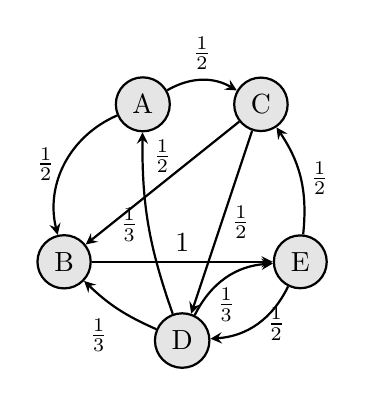
\begin{tikzpicture}[
        scale=0.5,
        ->,
        >=stealth,
        node distance=4cm,
        thick,
        main node/.style={circle, draw, fill=black!10, minimum size=4mm}
        ]

        % Nodes/States
        \node[main node] (A) at (0,4) {A};
        \node[main node] (B) at (-2,0) {B};
        \node[main node] (C) at (3,4) {C};
        \node[main node] (D) at (1,-2) {D};
        \node[main node] (E) at (4,0) {E};

        % Edges with reversed direction
        % From A to B (curving outwards)
        \path (A) edge [bend right=40] node[left] {$\frac{1}{2}$} (B);
        \path (A) edge [bend left=30] node[above] {$\frac{1}{2}$} (C);
        
        % From B to other states
        \path (C) edge node[above] {$\frac{1}{2}$} (B);
        \path (D) edge [bend left=10] node[below left] {$\frac{1}{3}$} (B);
        \path (D) edge [bend left=10] node[left] {$\frac{1}{3}$} (A);
        
        % From E to C (corrected direction)
        \path (E) edge [bend right=20] node[right] {$\frac{1}{2}$} (C);
        
        % From D to other states
        \path (C) edge  node[right] {$\frac{1}{2}$} (D);
        \path (D) edge [bend left=30] node[below] {$\frac{1}{3}$} (E);
        
        % From E to other states
        \path (B) edge node[above] {$1$} (E);
        \path (E) edge [bend left=30] node[right] {$\frac{1}{2}$} (D);
      \end{tikzpicture}
    \end{subfigure}
    \hfill 
    \begin{subfigure}[b]{0.48\textwidth}
      \centering
      \begin{equation}
        \begin{pmatrix}0&0&0&\frac{1}{3}&0\\
        \frac{1}{2}&0&\frac{1}{2}&\frac{1}{3}&0\\
        \frac{1}{2}&0&0&0&\frac{1}{2}\\
        0&0&\frac{1}{2}&0&\frac{1}{2}\\
        0&1&0&\frac{1}{3}&0\end{pmatrix}
      \end{equation}
    \end{subfigure}
    \caption{Markov chain graph and corresponding adjacency/transition matrix.}
    \label{fig:markov_chain}
  \end{figure}

  However, the theorem above requires the matrix to be strictly positive, which is often not true for Markov chains in general. This theorem does not hold true in the following example, 
  \begin{equation}
    A = \begin{pmatrix}
    0&0&0&\frac{1}{3} \\
    \frac{1}{2}&0&0&\frac{1}{3} \\
    0&0&0&\frac{1}{3} \\
    \frac{1}{2}&0&0&0
    \end{pmatrix} \implies A^{1000} 
        \begin{pmatrix}
    \frac{1}{4} \\ \frac{1}{4} \\ \frac{1}{4} \\ \frac{1}{4}
    \end{pmatrix} = 
        \begin{pmatrix}
    0 \\ 9/20 \\ 11/20 \\ 0
    \end{pmatrix}, \; A^{1001} 
        \begin{pmatrix}
    \frac{1}{4} \\ \frac{1}{4} \\\frac{1}{4} \\ \frac{1}{4}
    \end{pmatrix} = 
        \begin{pmatrix}
    0 \\ 11/20 \\ 9/20 \\ 0
    \end{pmatrix}
  \end{equation}
  That is, $A^N v$ oscillates between these two values. Furthermore, given three notes $A, B, C$ as such

  \begin{figure}[H]
    \centering 
    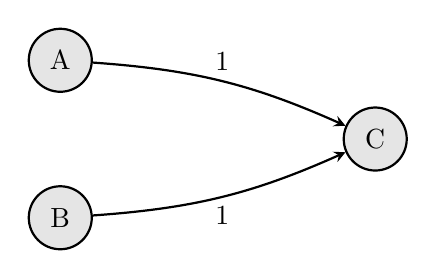
\begin{tikzpicture}[
      ->,
      >=stealth,
      node distance=3cm,
      thick,
      main node/.style={circle, draw, fill=black!10, minimum size=8mm}
      ]
      % Nodes
      \node[main node] (A) at (0,2) {A};
      \node[main node] (B) at (0,0) {B};
      \node[main node] (C) at (4,1) {C};

      % Edges with weight labels
      \path (A) edge [bend left=10] node[above] {$1$} (C);
      \path (B) edge [bend right=10] node[below] {$1$} (C);
    \end{tikzpicture}
    \label{fig:degenerate_markov_chain}
  \end{figure}
  the entries of the adjacency matrix is not well-defined. 
  \begin{equation}
     \begin{pmatrix} 0&0&? \\0&0&? \\1&1&?\end{pmatrix}
  \end{equation}
  Google CEO Larry Page actually developed a solution by implementing what he called a \textit{dampening factor}. Given stochastic matrix $B_{i j} = \frac{1}{N}$, he redefined the chain to be 
  \begin{equation}
    M = \alpha A + (1-\alpha) B, \; 0< \alpha < 1
  \end{equation}
  It is clear that $M$ is now a strictly positive stochastic matrix. The $\alpha$ is the dampening factor, and its optimal value is known to be about $0.67$. The value of the alpha determines how much of the data is "washed away." When $\alpha = 0$, none of the data is lost, and when $\alpha = 1$, all of the data is lost. 

  Due to the limitations of Perron's theorem, we can extend it with the following.

  \begin{theorem}[Frobenius Extension to Perron]
  Any $n \times n$ matrix $F \geq 0$, $F \neq 0$ has eigenvalue $\lambda$ such that
  \begin{enumerate}
      \item $\lambda \geq 0$ and $F h = \lambda h$, $h\geq 0$ \item every eigenvalue $\kappa$ satisfies: $|\kappa| \leq \lambda$ 
      \item if $|\kappa| = \lambda$, then 
      \begin{equation}
        \kappa = e^{\frac{2 \pi i k}{m}} \lambda, \; k, m \in \mathbb{Z}_+, \; m \leq n
      \end{equation}
  \end{enumerate}
  \end{theorem}

\subsection{Duality Theorem}

  In this section we will denote vector inequalities as entry-wise inequalities.Recall that elements of a vector space $X$ can be interpreted as column vectors, and elements of the dual of the vector space $X^\ast$ can be interpreted as row vectors. Therefore, value of $\phi$ at $x$ is denoted
  \begin{equation}
    \phi (x) = \phi_1 x_1 + \phi_2 x_2 + ... + \phi_n x_n
  \end{equation}
  Furthermore, the dual of $X^\ast$ is $X$ itself, and given that $Y$ is a linear subspace of $X$, the annihilator of $Y^\perp$ is $Y$. 
  \begin{equation}
    X = X^{**}, \;\; Y = Y^{\perp\perp}
  \end{equation}
  Suppose $Y$ is defined as the linear space spanned by the $m$ vectors $y_1, y_2, ..., y_m$ in $X$. That is, $Y$ consists of all vectors $y$ of the form
  \begin{equation}
    y = \sum_{j=1}^m a_j y_j
  \end{equation}
  It is clear by linearity that $\phi$ belongs to $Y^\perp$ if and only if
  \begin{equation}
    \phi (y_j) = 0, \;\; j = 1, 2, ..., m
  \end{equation}
  That is, a vector $y$ can be written as a linear combination of $m$ given vectors $y_j$ if and only if every $\phi$ that annihilates the $m$ vectors a also annihilates $0$. Now, we state a theorem that allows us to check if a vector $y$ can be written as a \textit{nonnegative} linear combinations of the $y_j$s. 

  \begin{theorem}
  A vector $y$ can be written as a linear combination of given vectors $y_j$ with nonnegative coefficients if and only if every $\zeta \in X^\ast$ that satisfies 
  \begin{equation}
     \zeta (y_j) \geq 0, \;\; j = 1, 2, ..., m
  \end{equation}
  also satisfies 
  \begin{equation}
    \zeta (y) \geq 0
  \end{equation}
  \end{theorem}
  \begin{proof}
  The proof is not the easiest to construct rigorously, but it can be visualized easily. 
  \end{proof}

  \begin{corollary}
  Given a $n \times m$ matrix $Y$, a vector $y$ with $n$ components can be written in the form 
  \begin{equation}
    y = Y p, \;\; p \geq 0
  \end{equation}
  if and only if every row vector $\zeta$ that satisfies 
  \begin{equation}
    \zeta Y \geq 0
  \end{equation}
  also satisfies 
  \begin{equation}
    \zeta y \geq 0
  \end{equation}
  \end{corollary}

  \begin{theorem}
  Given an $n \times m$ matrix $Y$ and a column vector $y$ with $n$ components, the inequality 
  \begin{equation}
    y \geq Y p, \;\; p \geq 0
  \end{equation}
  is satisfied if and only if every $\zeta$ that satisfies
  \begin{equation}
    \zeta Y \geq 0, \;\; \zeta \geq 0
  \end{equation}
  also satisfies 
  \begin{equation}
    \zeta y \geq 0
  \end{equation}
  \end{theorem}

  \begin{theorem}[Duality Theorem]
  Let $Y$ be a given $n \times m$ matrix, $y$ a given column vector with $n$ components, and $\gamma$ a given row vector with $m$ components. Let 
  \begin{equation}
    S = \sup_p \{\gamma p\}
  \end{equation}
  for all column vectors $p$ with $m$ components satisfying $y \geq Y p, \; p \geq 0$. A well-defined such $p$ is called \textbf{supremum admissible}. Additionally, let 
  \begin{equation}
    s = \inf_\zeta \{ \zeta y\}
  \end{equation}
  for all row vectors $\zeta$ with $n$ components satisfying $\gamma \leq \zeta Y, \; \zeta \geq 0$. A well-defined such $\zeta$ is called \textbf{infimum admissible}. Given that admissible vectors $p$ and $\zeta$ exist, then $S$ and $s$ are finite and 
  \begin{equation}
    S = s
  \end{equation}
  \end{theorem}

\subsection{Alternating Sign Matrices}

  We now describe a generalization of permutation matrices. While these kinds of matrices haven't been studied deeply, its applications lie in measuring the computational complexity of the Dodgson Condensation method for computing matrix determinants. The set of alternating sign matrices also forms a bijection with combinatorial objects, such as plane partitions, aztec diamonds, ice models, etc. 

  \begin{definition}
  A matrix with elements $0, -1, 1$ where nonzero entries must alternate in the following pattern: $1, -1, 1, ..., -1, 1$ (i.e. begin and end with $1$) is called an \textbf{alternating sign matrix}. This means that every row and column must add up to $1$. 
  \end{definition}

  \begin{example}
  The following are alternating sign matrices. 
  \[\begin{pmatrix}
  0&1&0&0\\1&-1&0&1\\0&1&0&0\\0&0&1&0
  \end{pmatrix}, \begin{pmatrix}
  0&1&0\\1&-1&1\\0&1&0
  \end{pmatrix}\]
  \end{example}

  As with permutation matrices, we would like to calculate how many $n \times n$ alternating sign matrices there are for a given $n$. Let the set of all $n \times n$ alternating sign matices be denoted
  \begin{equation}
    \text{ASM}(n)
  \end{equation}

  \begin{proposition}[Alternating Sign Matrix Conjecture (Proved)]
  The number of $n \times n$ alternating sign matrices is the following. 
  \begin{equation}
    \text{card ASM}(n) = \prod_{k=0}^{n-1} \frac{(3k+1)!}{(n+k)!}
  \end{equation}
  \end{proposition}

  We now define a bijection between ASMs and another type of $n \times n$ matrix. Given $A \in \text{ASM}(n)$, we define $f: \text{ASM}(n) \longrightarrow \text{Mat}(n, \{0,1\})$ such that
  \begin{equation}
    \big(f(A)\big)_{ij} = \sum_{k=i}^n (a)_{kj}
  \end{equation}
  Basically, we leave the bottom row untouched and for each element on upper rows, we sum that element with all of the elements strictly below it. For example, 
  \[\begin{pmatrix}
  0&1&0&0\\1&-1&0&1\\0&1&0&0\\0&0&1&0
  \end{pmatrix} \mapsto \begin{pmatrix}
  1&1&1&1\\1&0&1&1\\0&1&1&0\\0&0&1&0
  \end{pmatrix}\]

  \begin{theorem}
  The set of matrices $\im(f) \subset \text{Mat}(n, \{0, 1\})$ is bijective to the set of $n \times n$ 6-vertex (or Ice-type) models, which are used to model crystal lattices for hydrogen bonds. 
  \end{theorem}

